\documentclass{article}
\usepackage[margin=1in]{geometry}
\usepackage{amsmath,amsfonts,amssymb}
\usepackage{listings}
\usepackage{color}
\usepackage{graphicx}
\usepackage{subfig}
\usepackage{blkarray}
\usepackage{multirow}
\usepackage{float}
\usepackage{caption}
\usepackage{subcaption}
\begin{document}
\begin{titlepage}
	\setlength{\parindent}{0pt}
	\large

\vspace*{-2cm}

\definecolor{dkgreen}{rgb}{0,0.6,0}
\definecolor{gray}{rgb}{0.5,0.5,0.5}
\definecolor{mauve}{rgb}{0.58,0,0.82}

\lstset{frame=tb,
  language=Python,
  aboveskip=3mm,
  belowskip=3mm,
  showstringspaces=false,
  columns=flexible,
  basicstyle={\small\ttfamily},
  numbers=none,
  numberstyle=\tiny\color{gray},
  keywordstyle=\color{blue},
  commentstyle=\color{dkgreen},
  stringstyle=\color{mauve},
  breaklines=true,
  breakatwhitespace=true,
  tabsize=3
}

University of Waterloo \par
CS 480 \par
\vspace{0.05cm}
r2knowle: 2023-11-13
\vspace{0.2cm}

{\huge Exercise \# 2 \par}
\hrule

\vspace{0.5cm}
\textbf{Q2b)} Below are the 4 graphs each documenting an aspect of the training and testing process for our VG11 net implimention:

\begin{tabular}{ll}

 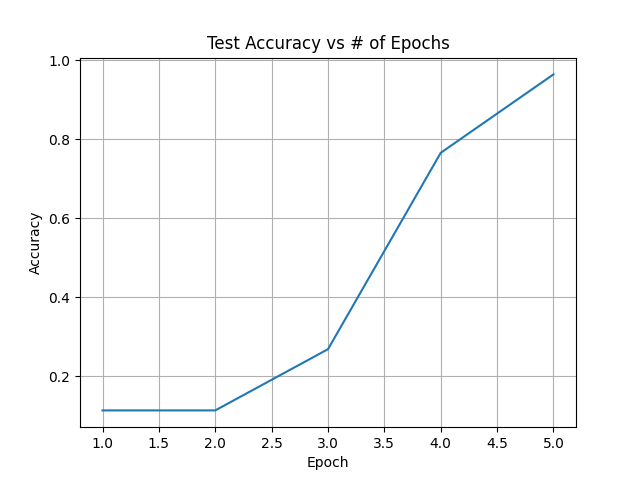
\includegraphics[width=.5\linewidth]{testA.png} &  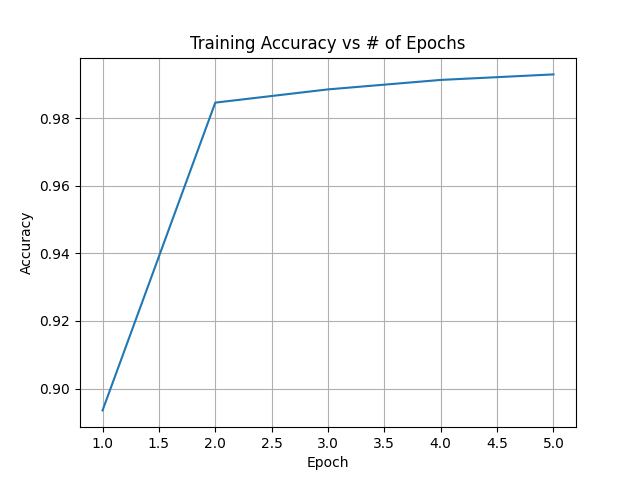
\includegraphics[width=.5\linewidth]{trainA.png}\\
 \hfil (i) Test accuracy vs the number of epochs \hfil & \hfil (ii) Training accuracy vs the number of epochs \hfil \\
 
  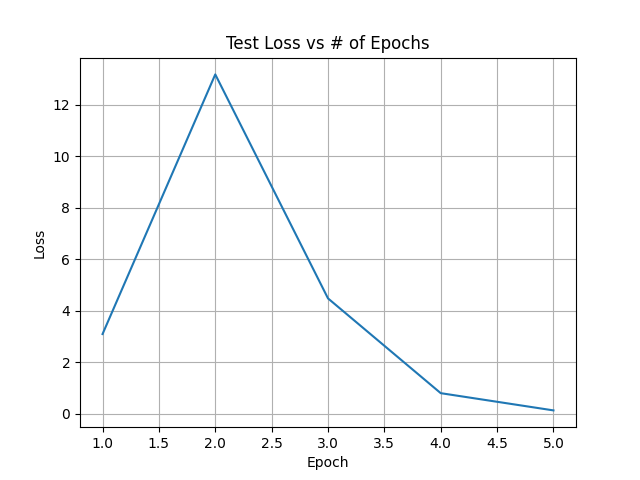
\includegraphics[width=.5\linewidth]{testL.png} &  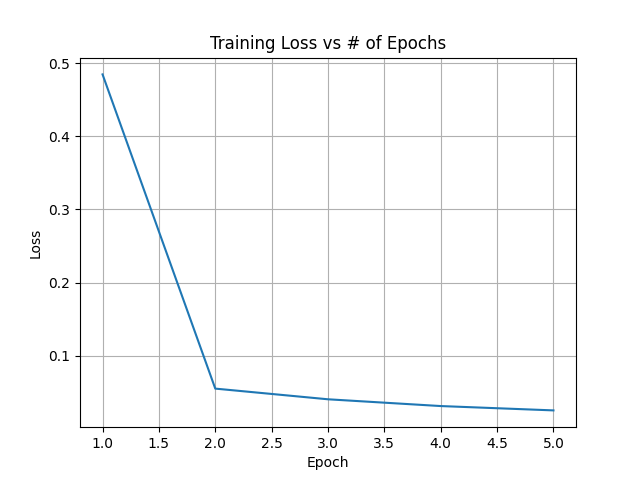
\includegraphics[width=.5\linewidth]{trainL.png}\\
 \hfil (i) Test loss vs the number of epochs \hfil & \hfil (ii) Training loss vs the number of epochs \hfil 
 
\end{tabular}
\newpage
\textbf{Q2ci)} Below we can see the testing accuracy across each flip:
\begin{center} 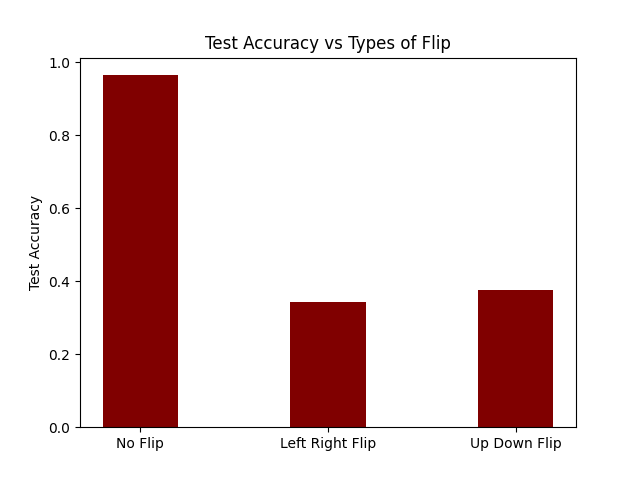
\includegraphics[width=0.7\linewidth]{flip.png} 
\end{center}
We can see that the updown flip has a higher testing accuracy then the left-right flip, this can be due to the fact that some digits remain more unchanged (like 3) from an updown flip then a right left flip. \textbf{Explict values are provided on the next page. } \\\\
\textbf{Q2cii)} Below we can see the testing accuracy across each flip:
\begin{center} 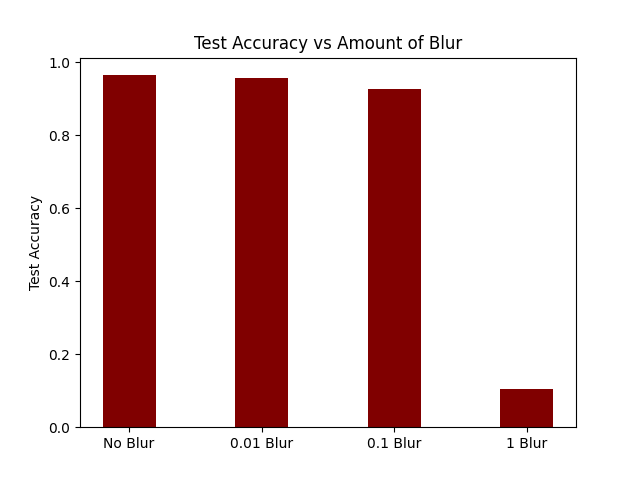
\includegraphics[width=0.7\linewidth]{blur.png} 
\end{center}
As the amount of blur increases, we can see that testing accuracy decreases. \textbf{Explict values are provided on the next page. }
\newpage
\textbf{Q2d)} By applying the both times of flips, and 0.01 and 0.1 blurring to our original dataset we can retrain for 5 epochs. After which we get the following graphs.\\
\begin{tabular}{ll}

 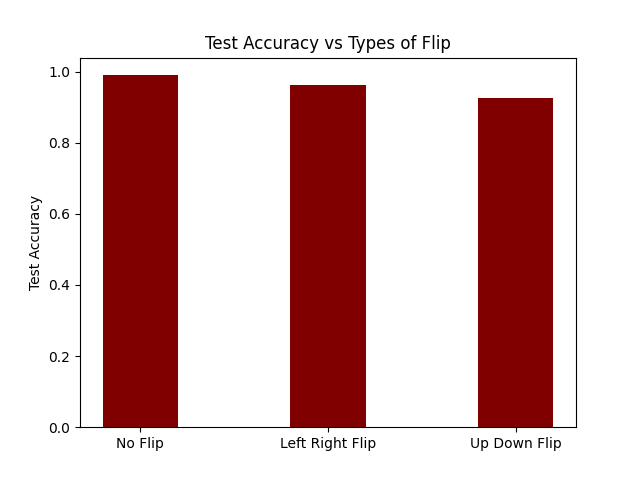
\includegraphics[width=.5\linewidth]{flip2.png} &  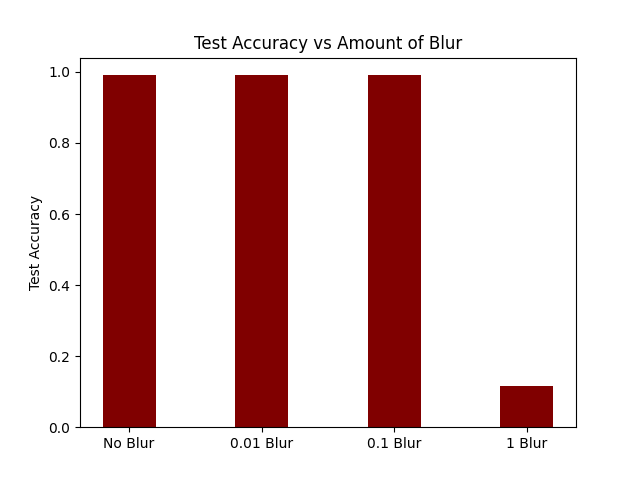
\includegraphics[width=.5\linewidth]{blur2.png}\\
 \hfil (i) Test accuracy vs flips \hfil & \hfil (ii) Training accuracy vs blur \hfil \\\\
 
\end{tabular}
We get the following updated test accuracies:
\begin{enumerate}
  \item No Flip / No Blur: 0.9899
  \item Left Right Flip: 0.9635
  \item Up Down Flip: 0.9255
  \item 0.01 Blur: 0.9905
  \item 0.1 Blur: 0.9907
  \item 1 Blur: 0.1159
\end{enumerate}
This is comparison to before we did the retraining where we had the following test accuracies:
\begin{enumerate}
  \item No Flip / No Blur: 0.9784
  \item Left Right Flip: 0.3481
  \item Up Down Flip: 0.3755
  \item 0.01 Blur: 0.9705
  \item 0.1 Blur: 0.9503
  \item 1 Blur: 0.1139
\end{enumerate}
\end{titlepage}
\end{document}